\chapter[Aplicaciones]{Aplicaciones}

A continuaci\'on se exponen los resultados de utilizar el paquete \textit{GPDPQuantReg} en R, mismo que, como se detalló en el cap\'itulo anterior, implementa el modelo \textit{GPDP} para la regresi\'on sobre cuantiles.

En primer lugar se presenta el ajuste del modelo en datos simulados, con el fin de comparar los resultados con los valores conocidos de antemano. Posteriormente se presenta para un conjunto de datos reales, con la intenci\'on de obtener conclusiones en aplicaciones pr\'acticas, mediante el uso del modelo central de esta tesis.

\section{Simulaci\'on}

Los datos de esta secci\'on se obtuvieron de la siguiente manera. Sea $y \in \mathbb{R}$ el valor de la variable de respuesta, $x \in \mathbb{R}$ su respectiva covariable, $g: \mathbb{R} \rightarrow \mathbb{R}$ la funci\'on denominada \textit{tendencia} y $E \in \mathbb{R}$ una dispersi\'on aleatoria, se simul\'o:
\begin{equation*}
    y = g(x) + E.
\end{equation*}
Las diferencias entre las subsecciones siguientes radican en variaciones del valor de $g$ y la distribuci\'on de $E$.

Dada esta construcci\'on, la funci\'on real del cuantil p-\textit{\'esimo} de $y|x$ se puede obtener como
\begin{equation*}
    q_p(y|x) = g(x) + q_p(E),
\end{equation*}
la cual se estimar\'a para diversos valores de $p$.

En todos los casos se ajust\'o el modelo para los cuantiles $0.5$\textit{-\'esimo}, por ser la mediana y una medida de tendencia central; el $0.95$\textit{-\'esimo}, dado que es un valor extremo, y el $0.25$\textit{-\'esimo}, debido a que es el primer cuartil, y no es ni medida de tendencia central, pero tampoco un valor extremo.

Por otro lado, para todos los casos se simularon 40 datos sin reemplazo, dentro del intervalo $(-15,15)$, con un refinamiento de 3 decimales.

\subsection{Tendencia simple, dispersi\'on simple}

Para obtener este conjunto de datos se utiliz\'o una tendencia $g$ considerada simple: la cuadr\'atica
\begin{equation*}
    g(x) = \frac{1}{40}x^2 - \frac{1}{20}x - 2.
\end{equation*}
Por otro lado, la distribuci\'on de la dispersi\'on $E \sim \mathcal{N}(0,1)$ tambi\'en fue sencilla, debido a que fue sim\'etrico y no acotado. Los datos simulados se pueden observar en la figura \ref{sample_sgse}.

Posteriormente se ajust\'o el modelo y se realiz\'o predicci\'on sobre un refinamiento del intervalo simulado de $x$, obteniendo buenos resultados (figura \ref{fitted_sgse}), ya que las funciones reales de los diversos cuantiles cayeron en su totalidad dentro del intervalo de probabilidad al 90\%, estimado por el modelo. Adem\'as, las medianas de la distribuciones posteriores siguieron un comportamiento similar a las originales.

\begin{figure}[H]
	\centering
	\caption{Datos simulados y cuantiles de referencia, para tendencia simple y dispersi\'on simple.}
	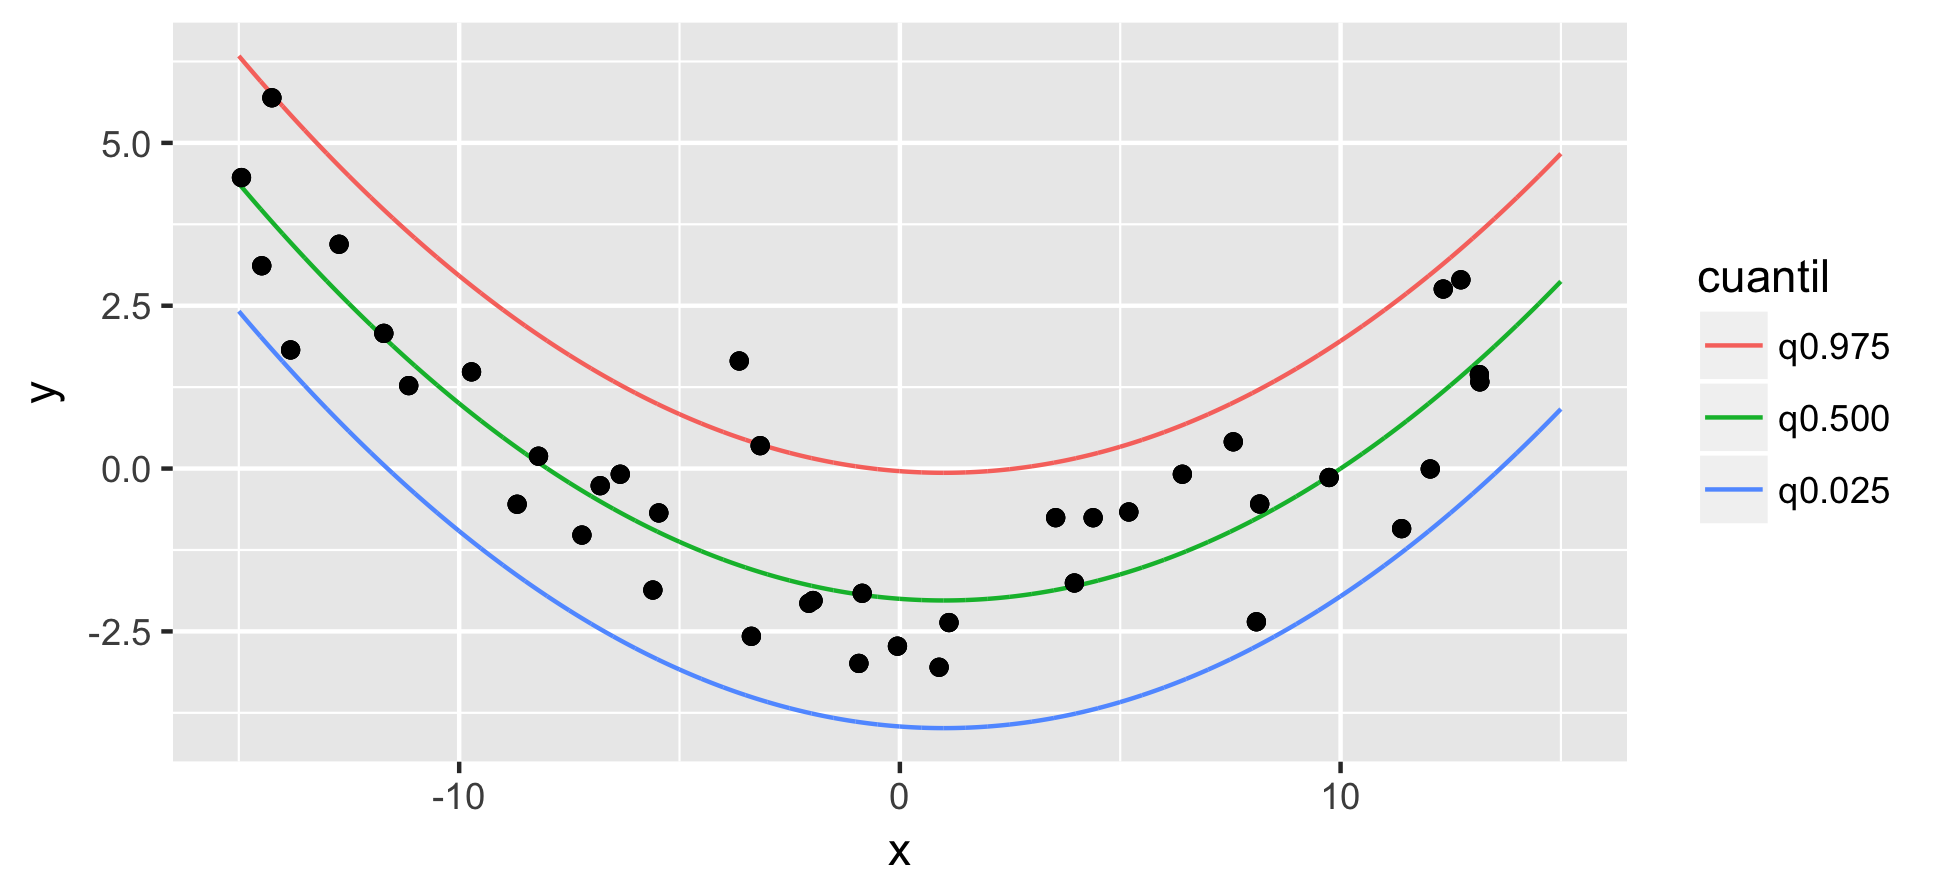
\includegraphics[width=0.60\textwidth]{Figures/Simulation/simple_g_simple_error/sample.png}
	\label{sample_sgse}
\end{figure}

\begin{figure}[H]
	\centering
	\caption{Ajuste del modelo \textit{GPDP}, para tendencia simple y dispersi\'on simple.}
	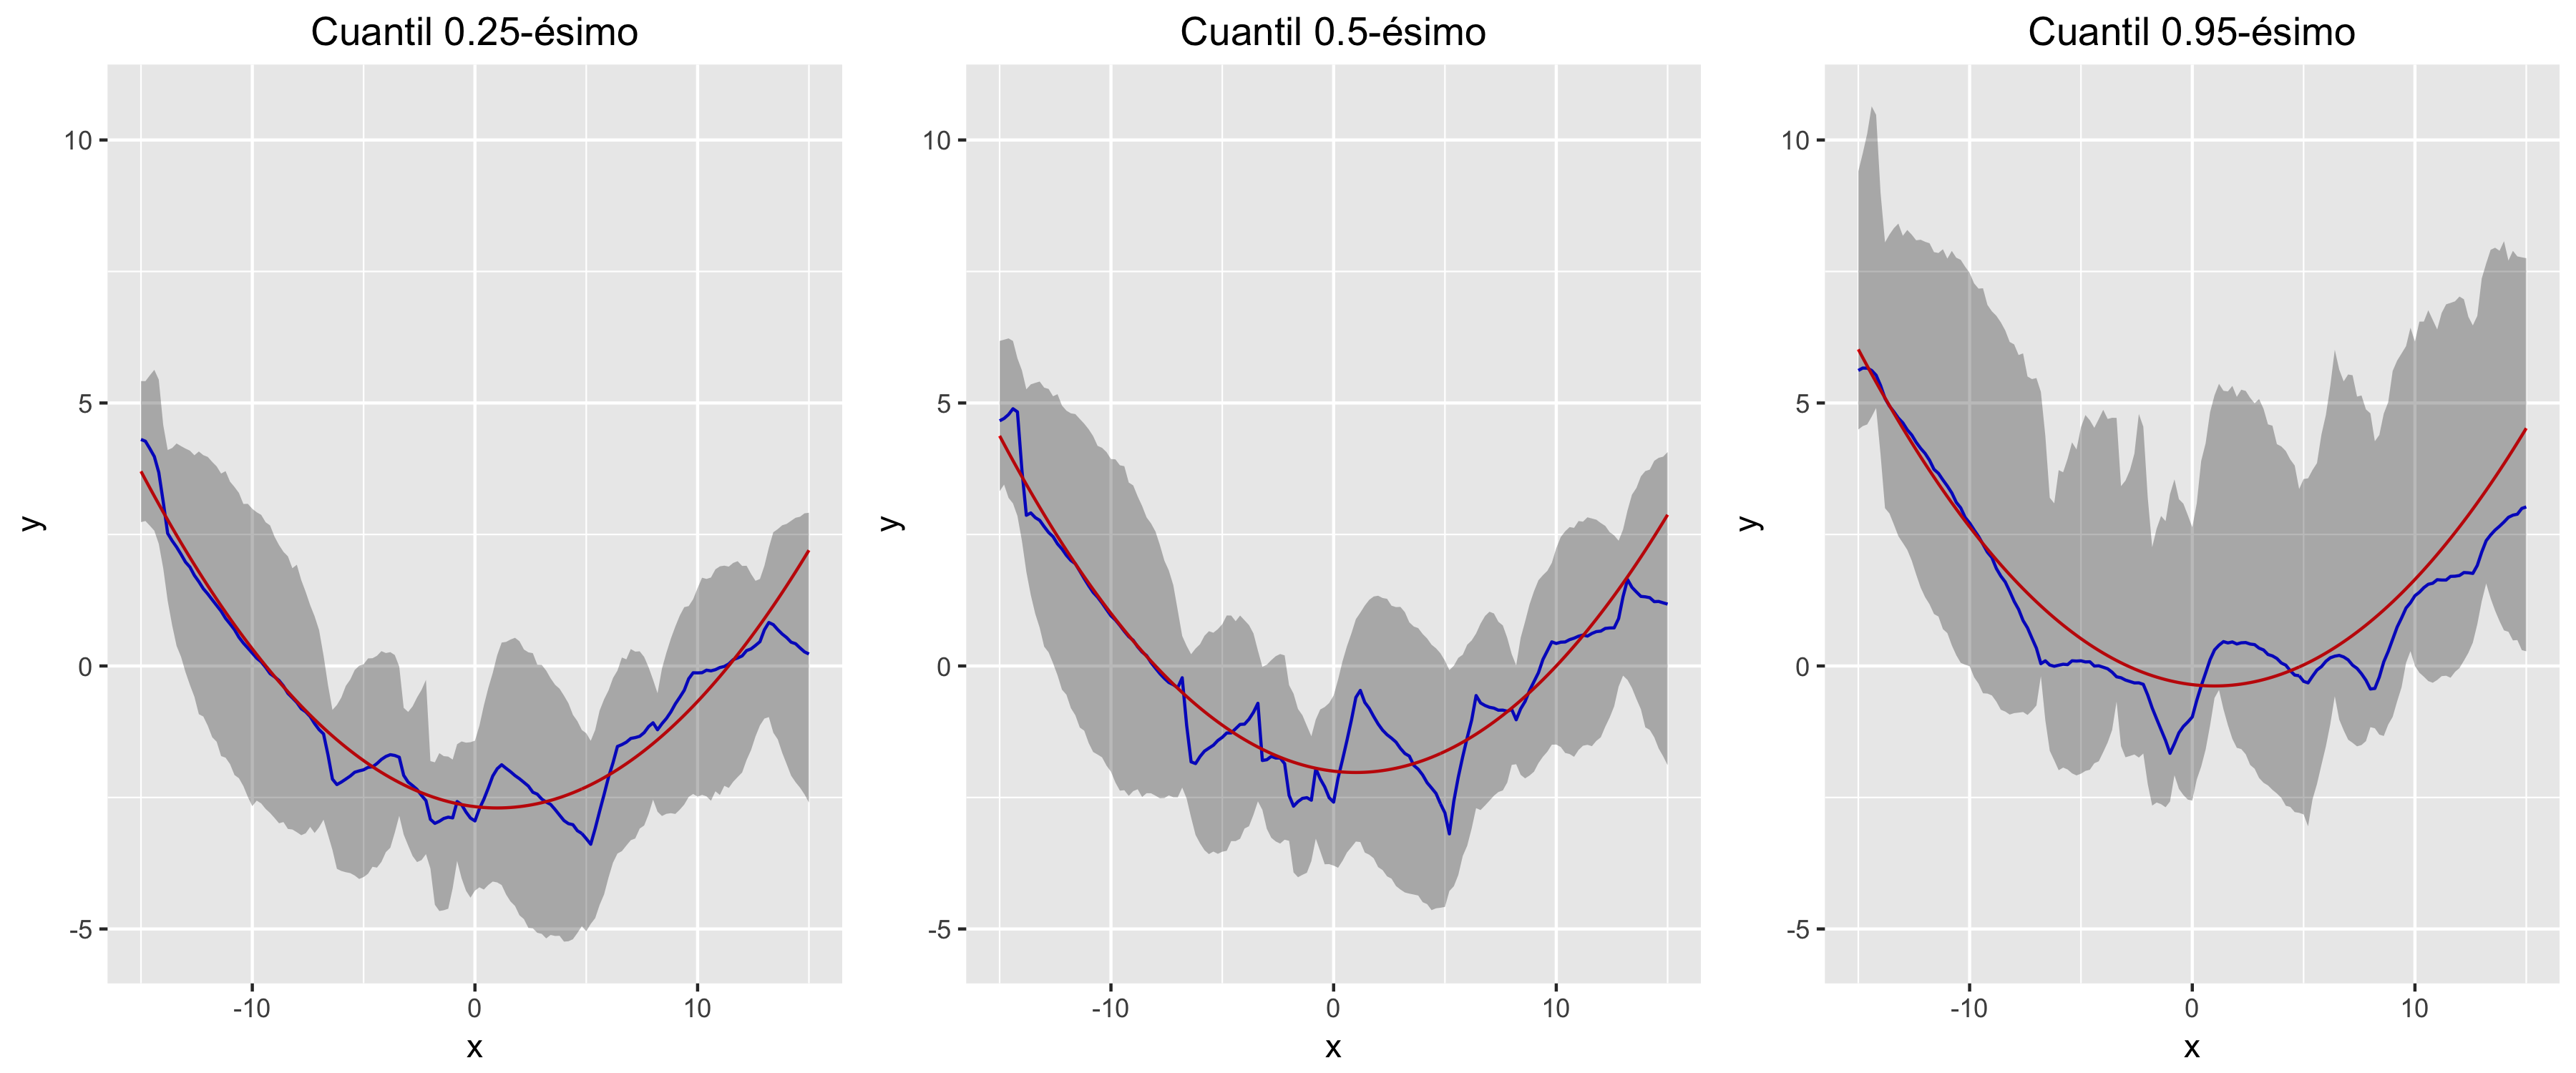
\includegraphics[width=\textwidth]{Figures/Simulation/simple_g_simple_error/fitted_models.png}
	\captionsetup{singlelinecheck=off,font=footnotesize}
    \caption*{Nota: La l\'inea roja representa el valor real de cada cuantil, la l\'inea azul representa la mediana de la distribuci\'on posterior predictiva y el \'area gris su intervalo de probabilidad al 90\%.}
	\label{fitted_sgse}
\end{figure}

Por otro lado, como se detall\'o en el cap\'itulo anterior, con el uso del paquete \textit{GPDPQuantReg} tambi\'en es posible algunos de los diagn\'osticos de las cadenas de Markov, los cuales se detallan en el \autoref{chap:MCMC}. Por ejemplo, se presentan los del cu\'antil $0.5$-\textit{\'esimo} en la figura \ref{diag_sgse}, mismos que reflejan un buen desempeño del algoritmo.

\begin{figure}[H]
	\centering
	\caption{Diagn\'osticos de las cadenas de Markov del cu\'antil $0.5$-\textit{\'esimo}, para tendencia simple y dispersi\'on simple.}
	\subfloat[Ergodicidad]{
	    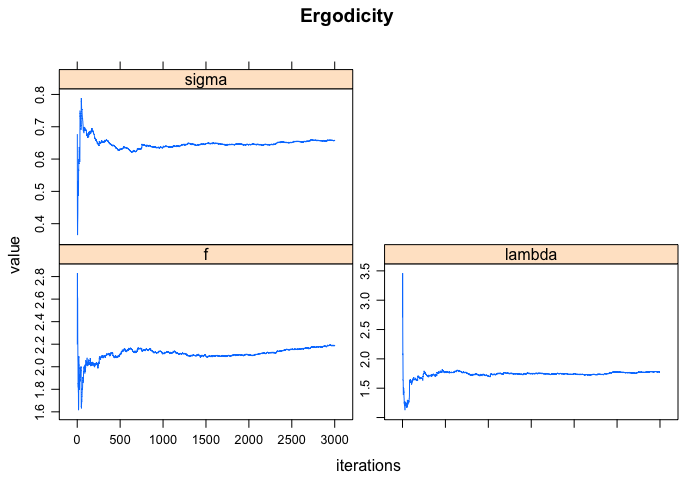
\includegraphics[width=0.45\textwidth]{Figures/Simulation/simple_g_simple_error/ergodicity.png}
	}
	\subfloat[Autocorrelaci\'on]{
	    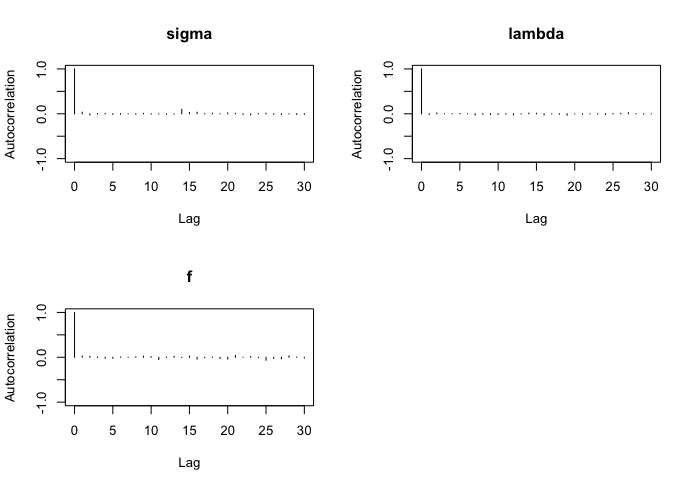
\includegraphics[width=0.45\textwidth]{Figures/Simulation/simple_g_simple_error/autocorrelation.png}
	}\\
	\subfloat[Correlaci\'on cruzada]{
	    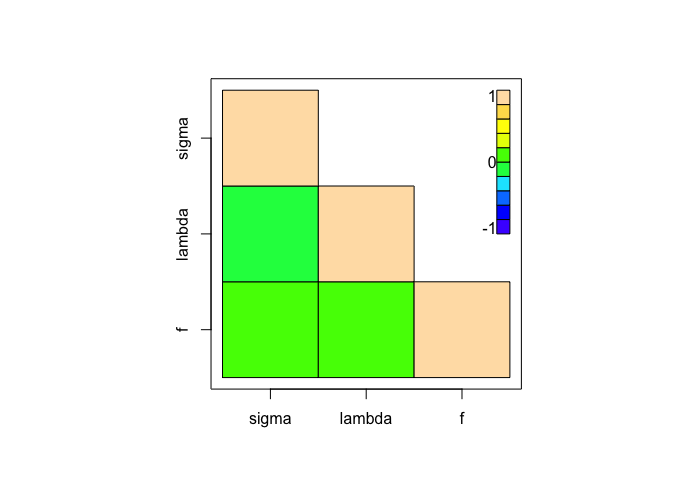
\includegraphics[width=0.45\textwidth]{Figures/Simulation/simple_g_simple_error/crosscorrelation.png}
	}
	\subfloat[Traza]{
	    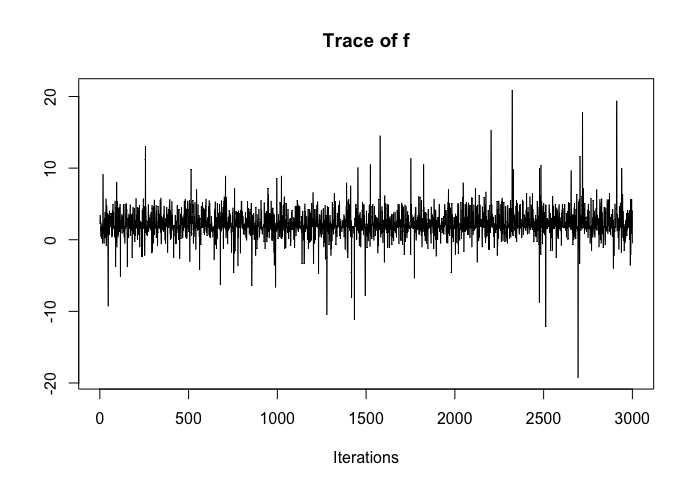
\includegraphics[width=0.45\textwidth]{Figures/Simulation/simple_g_simple_error/trace.png}
	}
	\label{diag_sgse}
\end{figure}

\subsection{Tendencia compleja, dispersi\'on simple}

En este caso, se mantuvo que $E \sim \mathcal{N}(1,0)$, pero la tendencia $g$ usada fue m\'as compleja:
\begin{equation*}
    g(x) = \frac{1}{2} x \cos(x) - \exp\left(\frac{1}{10}x\right).
\end{equation*}

Los datos simulados se pueden observar en la figura \ref{sample_cgse}, los cuales al ajustar el modelo mostraron de nuevo buenos resultados (figura \ref{fitted_cgse}), apareciendo la tendencia original adentro del intervalo de probabilidad al 90\% en pr\'acticamente todos los valores de $x$ en los que se realiz\'o predicci\'on, a excepci\'on de la \'ultima zona, en la que no hubo datos de entrenamiento.

\begin{figure}[H]
	\centering
	\caption{Datos simulados y cuantiles de referencia, para tendencia compleja y dispersi\'on simple.}
	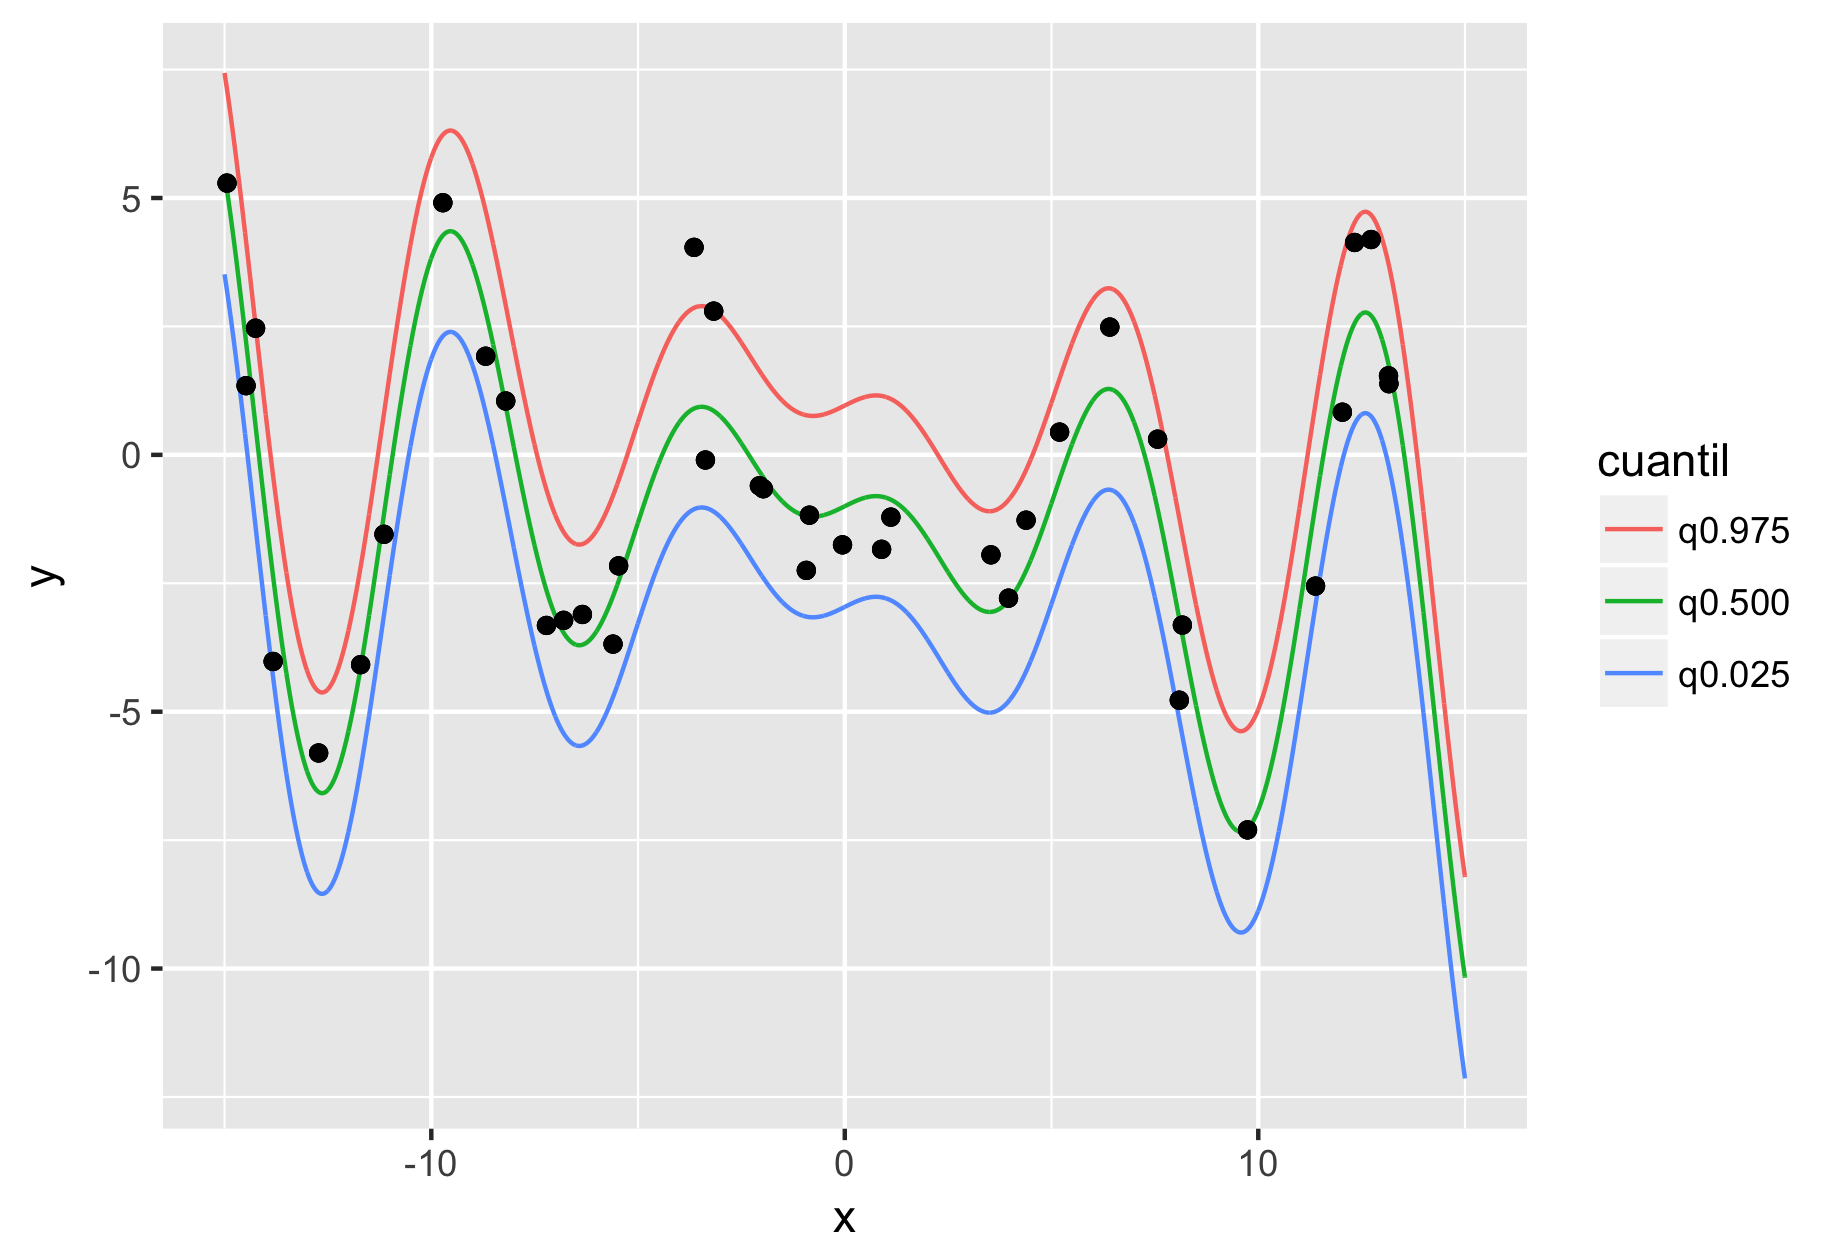
\includegraphics[width=0.60\textwidth]{Figures/Simulation/complex_g_simple_error/sample.png}
	\label{sample_cgse}
\end{figure}

\begin{figure}[H]
	\centering
	\caption{Ajuste del modelo \textit{GPDP}, para tendencia compleja y dispersi\'on simple.}
	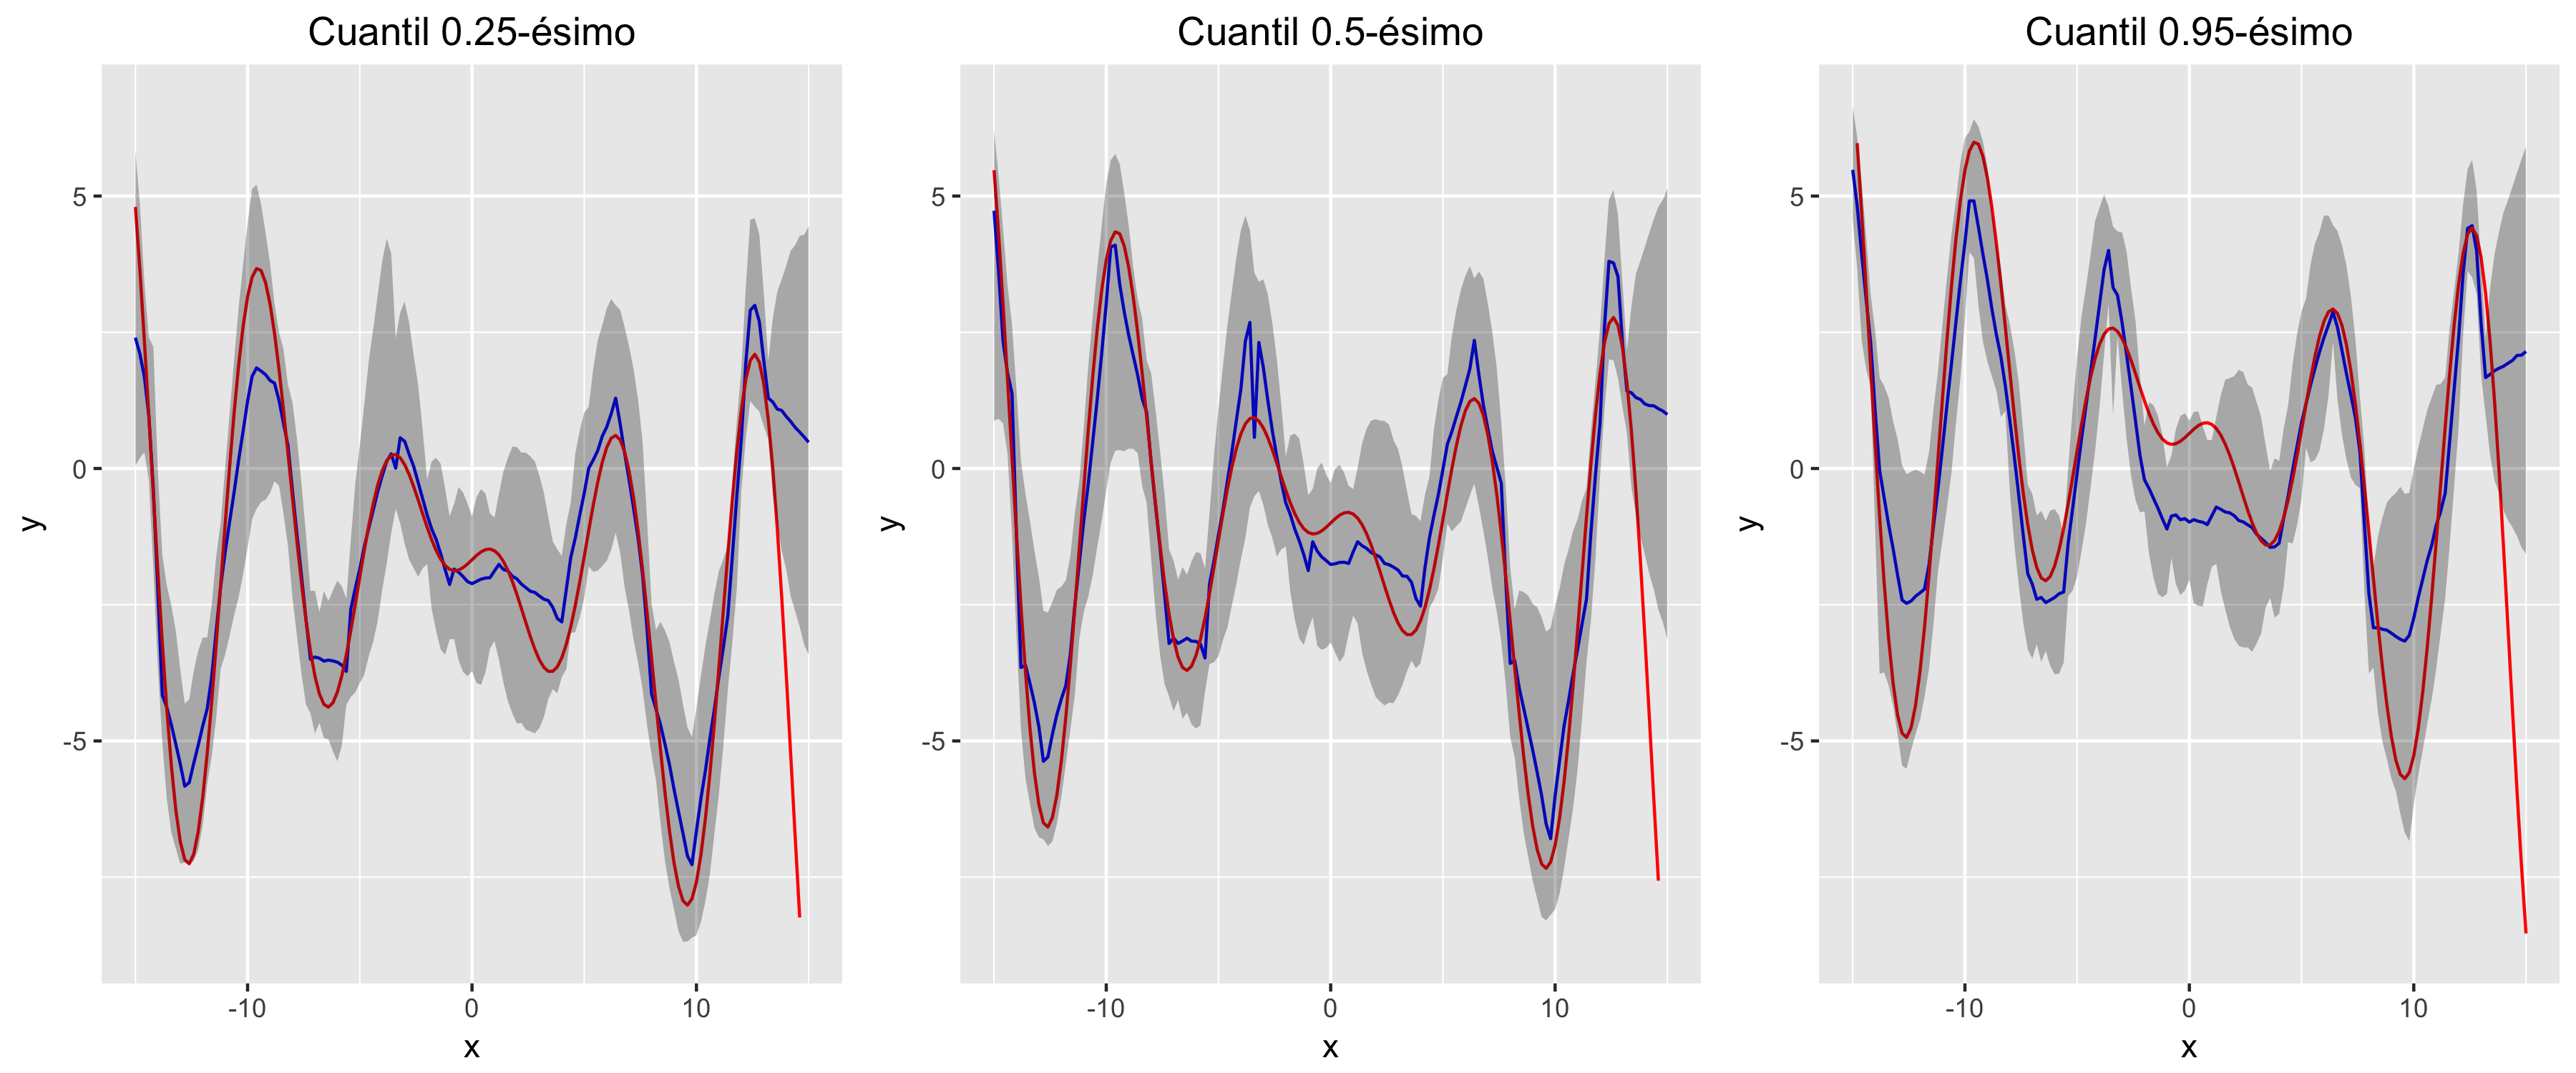
\includegraphics[width=\textwidth]{Figures/Simulation/complex_g_simple_error/fitted_models.png}
	\captionsetup{singlelinecheck=off, font=footnotesize}
    \caption*{Nota: La l\'inea roja representa el valor real de cada cuantil, la l\'inea azul representa la mediana de la distribuci\'on posterior predictiva y el \'area gris su intervalo de probabilidad al 90\%.}
	\label{fitted_cgse}
\end{figure}

\subsection{Tendencia simple, dispersi\'on compleja}

En este caso, se us\'o la tendencia lineal:
\begin{equation*}
    g(x) = \frac{1}{2} x.
\end{equation*}
La complejidad se introdujo en $E \sim \textit{Gamma}(\alpha = 2,\beta = 1)$, debido a que la dipersi\'on no fue sim\'etrica y fue acotada por la izquierda. 

El conjunto de datos usado para este modelo aparece en la figura \ref{sample_sgce}, y a pesar de la complejidad de la dispersi\'on, se obtuvieron buenos resultados (figura \ref{fitted_sgce}), debido a que nuevamente las funciones reales de los diversos cuantiles cayeron en su totalidad dentro del intervalo de probabilidad al 90\%, estimado por el modelo.

Un detalle notable es que, al igual que el caso de tendencia simple y dispersi\'on simple, la estimaci\'on de la funci\'on del cuantil 0.95\textit{-\'esimo} muestra una varianza m\'as grande que los otros dos cuantiles. Esto debido a que en valores extremos el modelo refleja mayor incertidumbre de lo que en realidad podr\'ia estar ocurriendo.

\begin{figure}[H]
	\centering
	\caption{Datos simulados y cuantiles de referencia, para tendencia simple y dispersi\'on compleja.}
	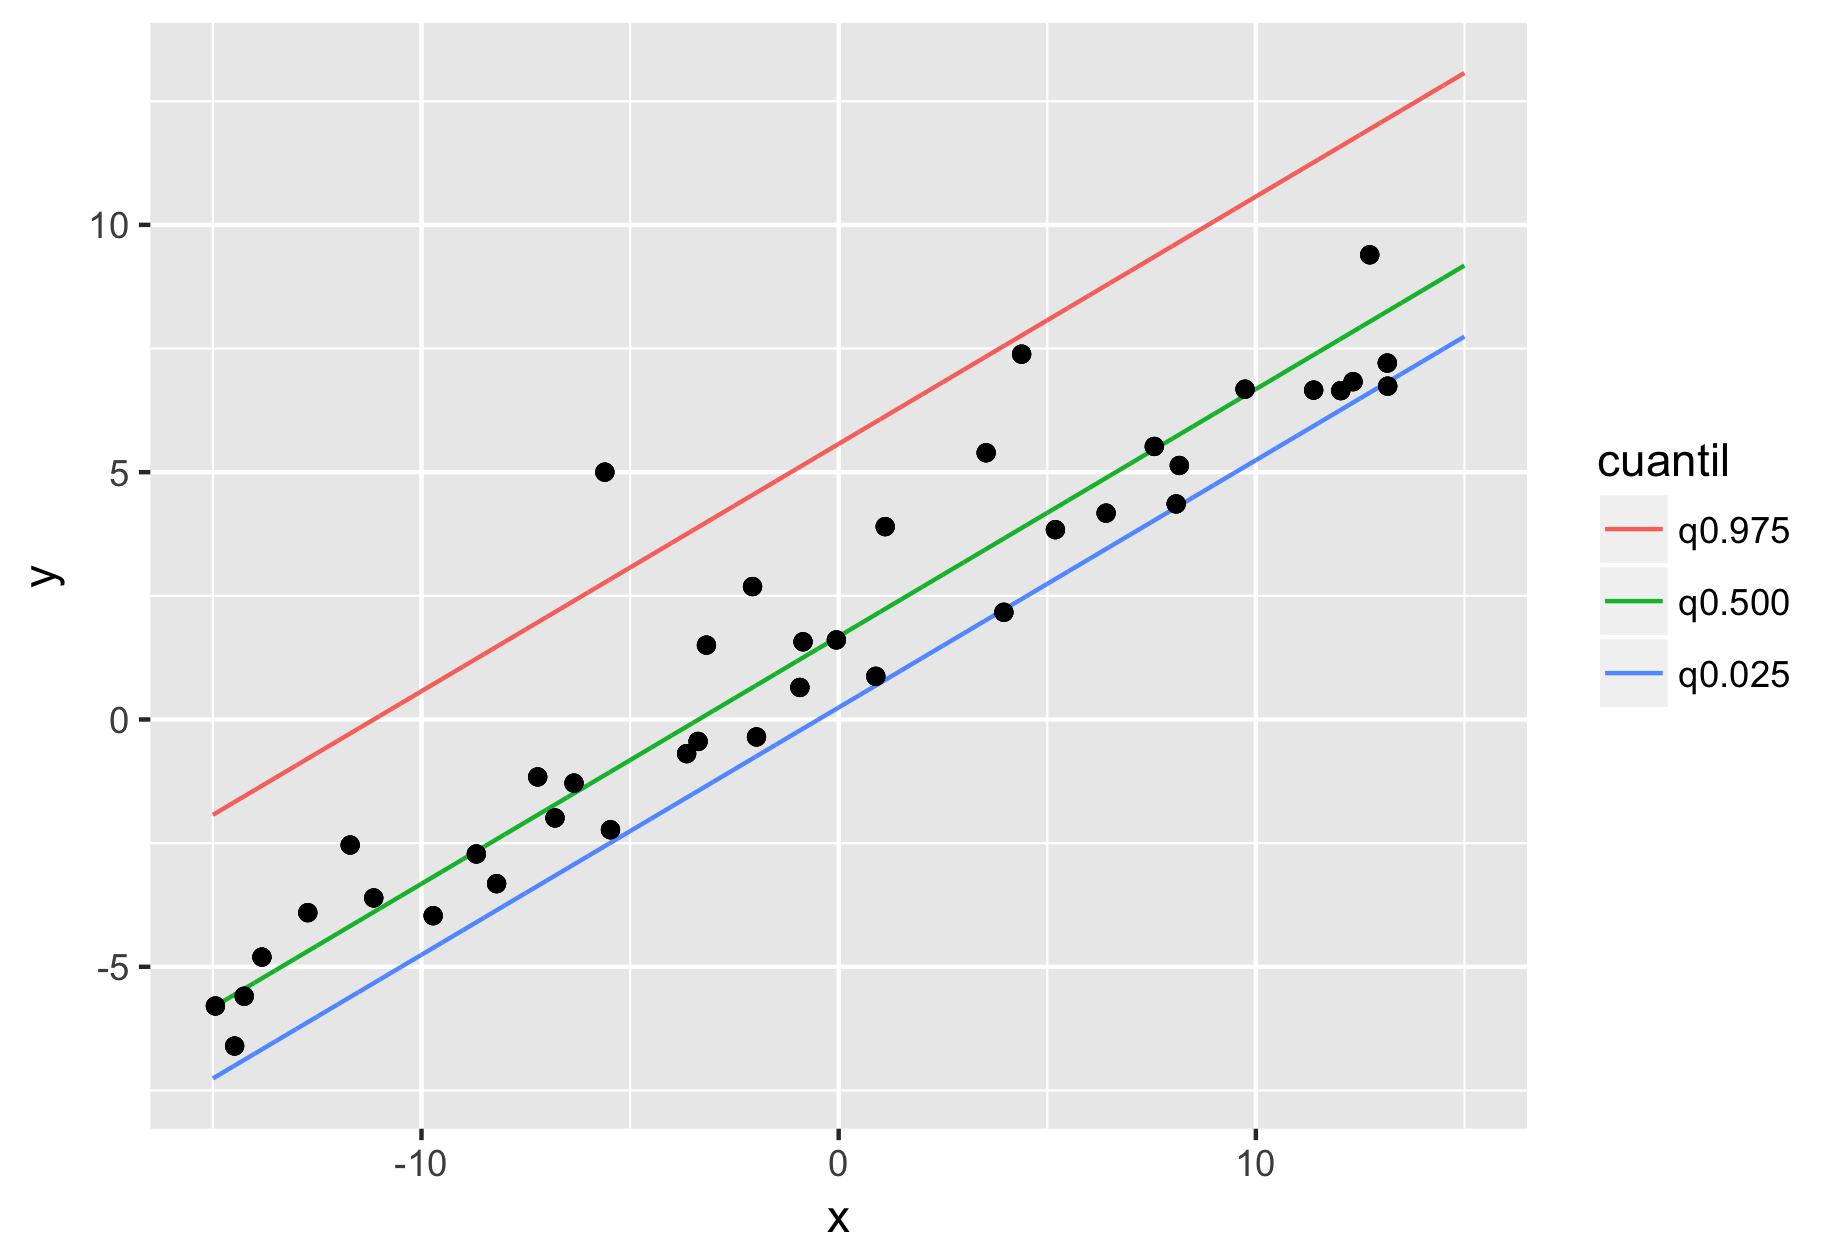
\includegraphics[width=0.60\textwidth]{Figures/Simulation/simple_g_complex_error/sample.png}
	\label{sample_sgce}
\end{figure}

\begin{figure}[H]
	\centering
	\caption{Ajuste del modelo \textit{GPDP}, para tendencia simple y dispersi\'on compleja.}
	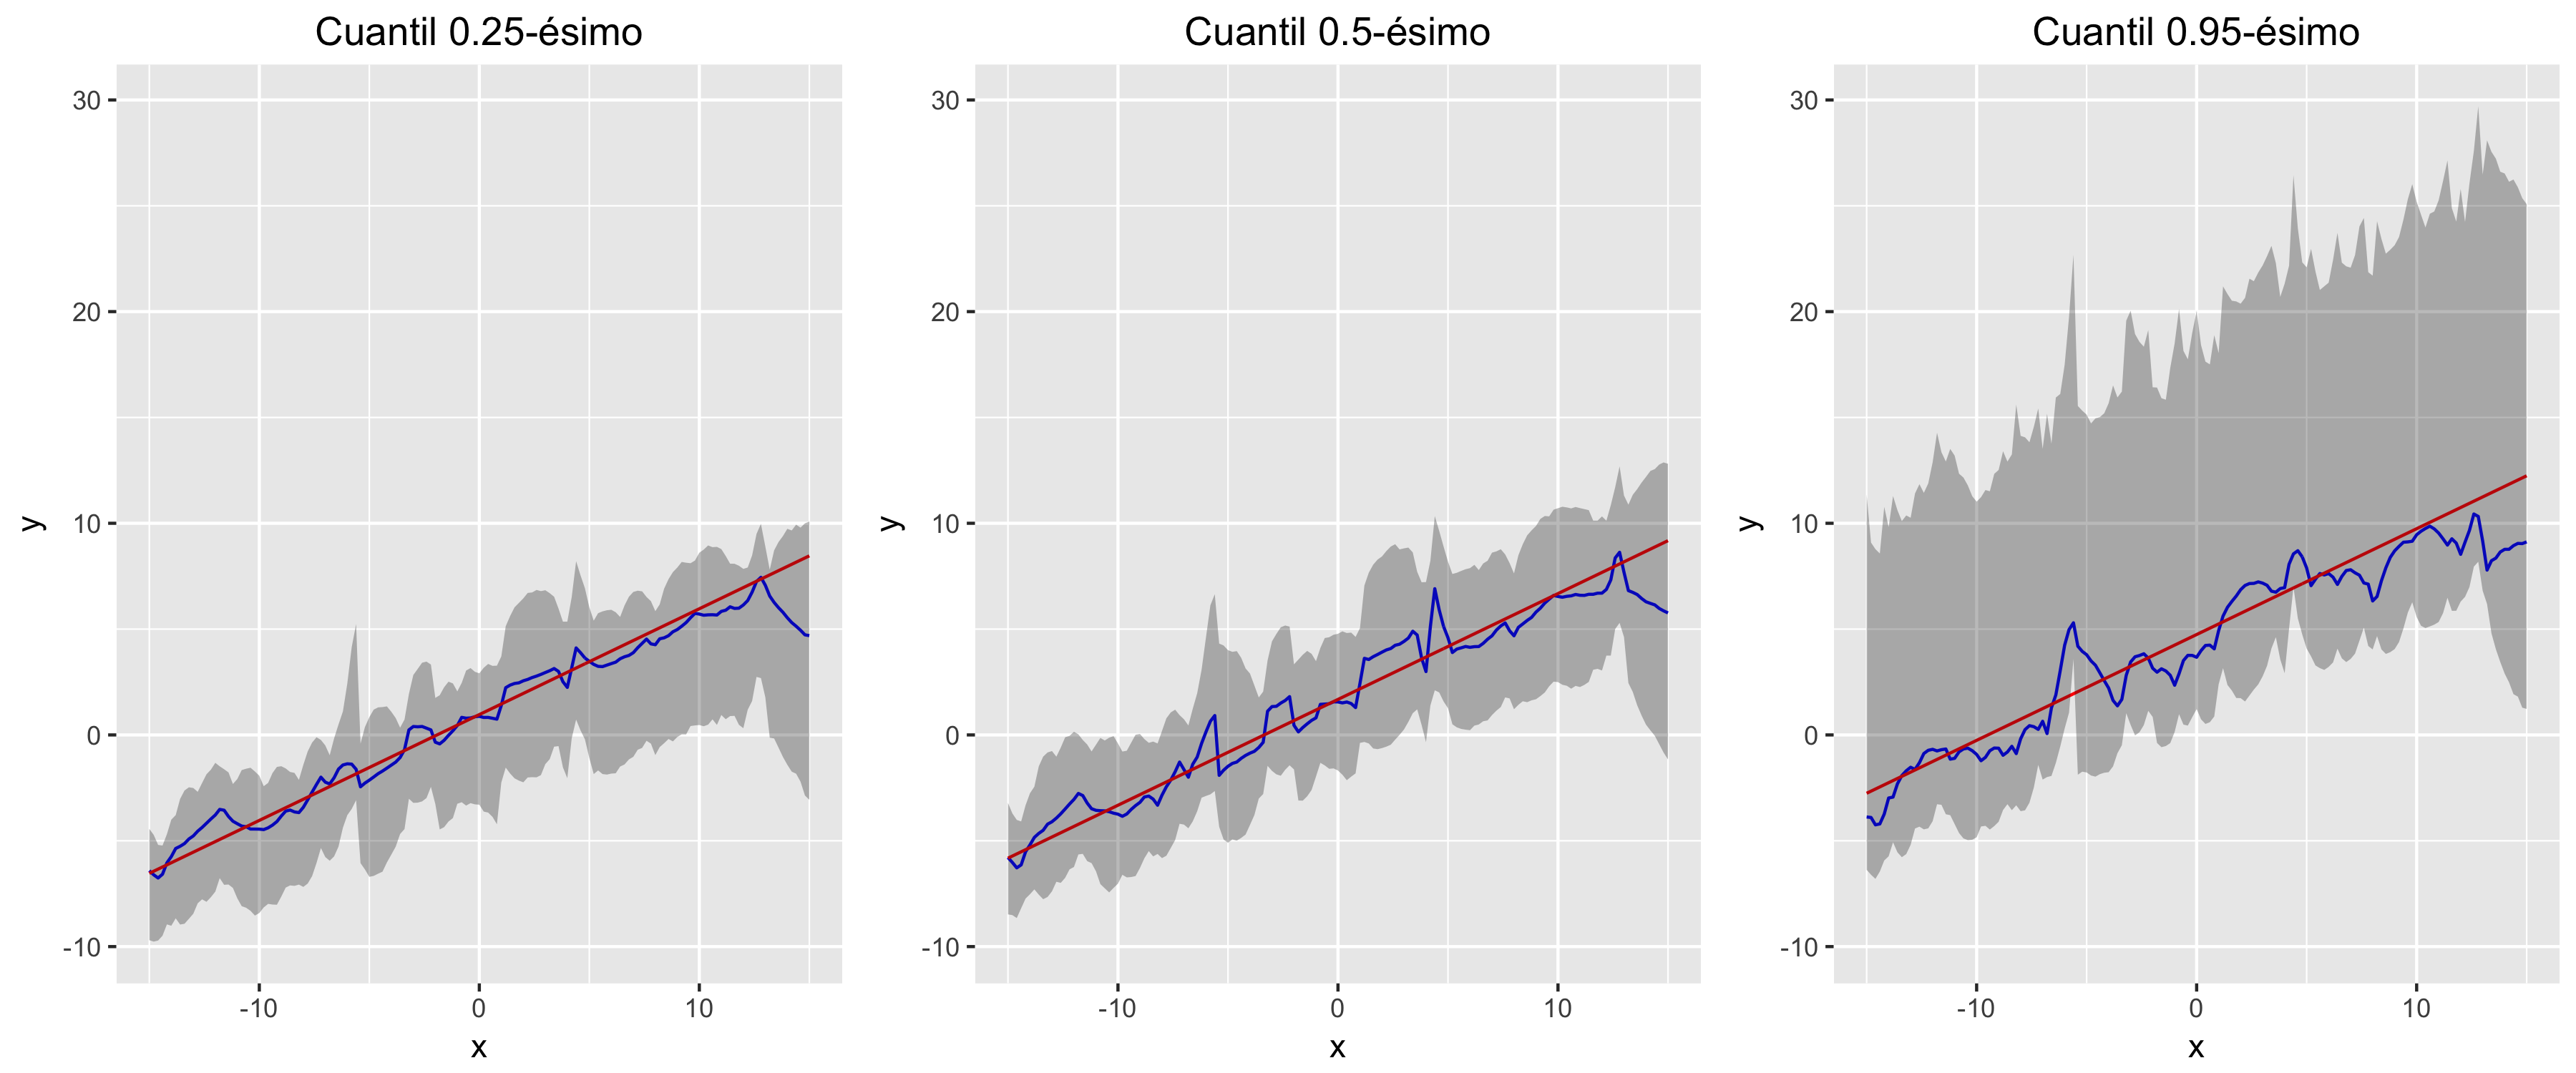
\includegraphics[width=\textwidth]{Figures/Simulation/simple_g_complex_error/fitted_models.png}
	\captionsetup{singlelinecheck=off,font=footnotesize}
    \caption*{Nota: La l\'inea roja representa el valor real de cada cuantil, la l\'inea azul representa la mediana de la distribuci\'on posterior predictiva y el \'area gris su intervalo de probabilidad al 90\%.}
	\label{fitted_sgce}
\end{figure}

\subsection{Tendencia compleja, dispersi\'on compleja}

En este modelo se usaron datos (figura \ref{sample_cgce}) provenientes tanto de una dispersi\'on compleja, $E \sim \textit{Gamma}(\alpha = 2,\beta = 1)$, como de una tendencia $g$ compleja:
\begin{equation*}
    g(x) = \frac{1}{2} x \cos(x) - \exp\left(\frac{1}{10}x\right).
\end{equation*}

Despu\'es del ajuste (figura \ref{fitted_cgce}), el balance fue positivo, debido a que las funciones reales de los diversos cuantiles cayeron en su totalidad dentro del intervalo de probabilidad al 90\%, del estimado por el modelo, a excepci\'
on de la zona de la que no se tuvieron datos, como en el caso de tendencia compleja y dispersi\'on simple. Pero a diferencia de ese modelo, la dispersi\'on compleja produce una mayor incertidumbre, particularmente notoria en el caso del cuantil 0.95\textit{-\'esimo}.

\begin{figure}[H]
	\centering
	\caption{Datos simulados y cuantiles de referencia, para tendencia compleja y dispersi\'on compleja.}
	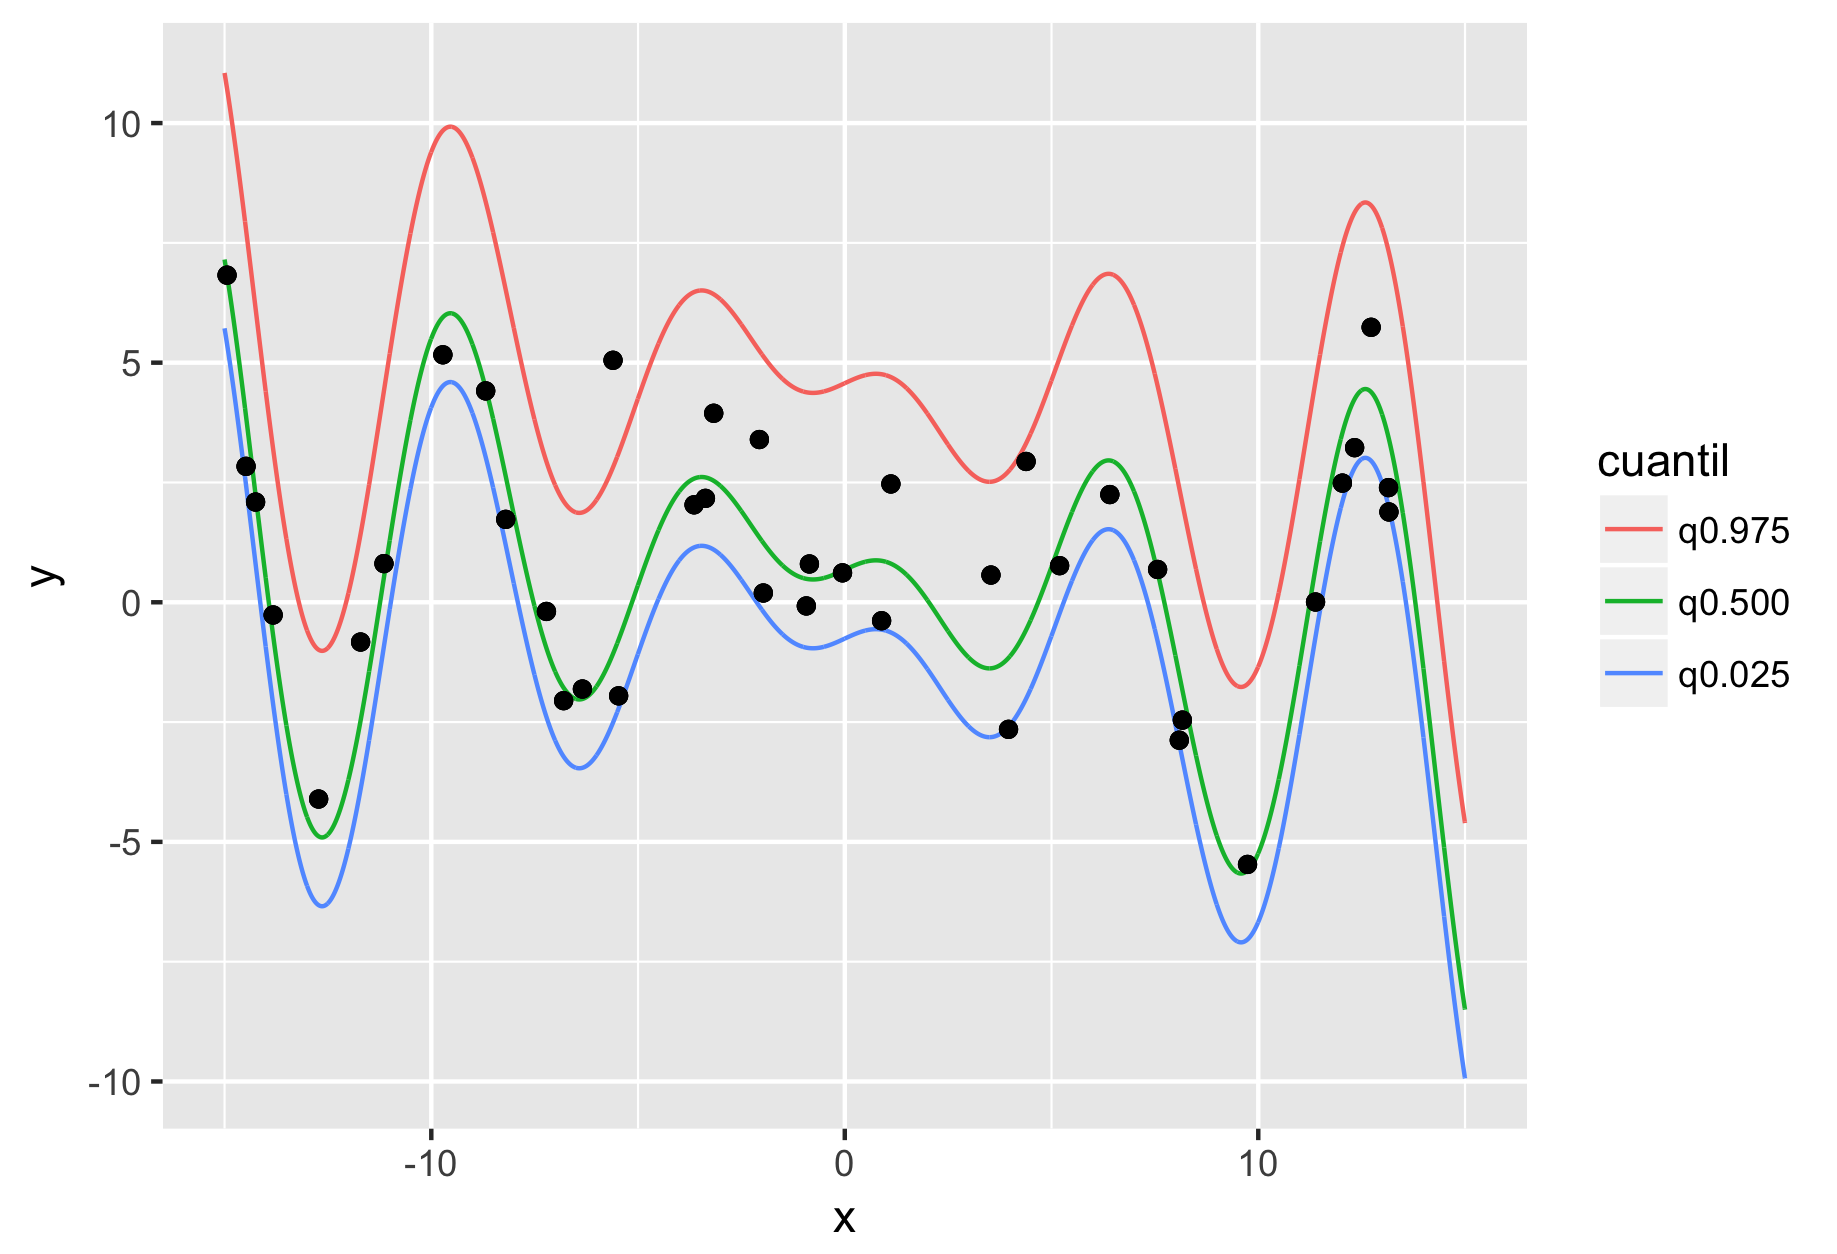
\includegraphics[width=0.60\textwidth]{Figures/Simulation/complex_g_complex_error/sample.png}
	\label{sample_cgce}
\end{figure}

\begin{figure}[H]
	\centering
	\caption{Ajuste del modelo \textit{GPDP}, para tendencia compleja y dispersi\'on compleja.}
	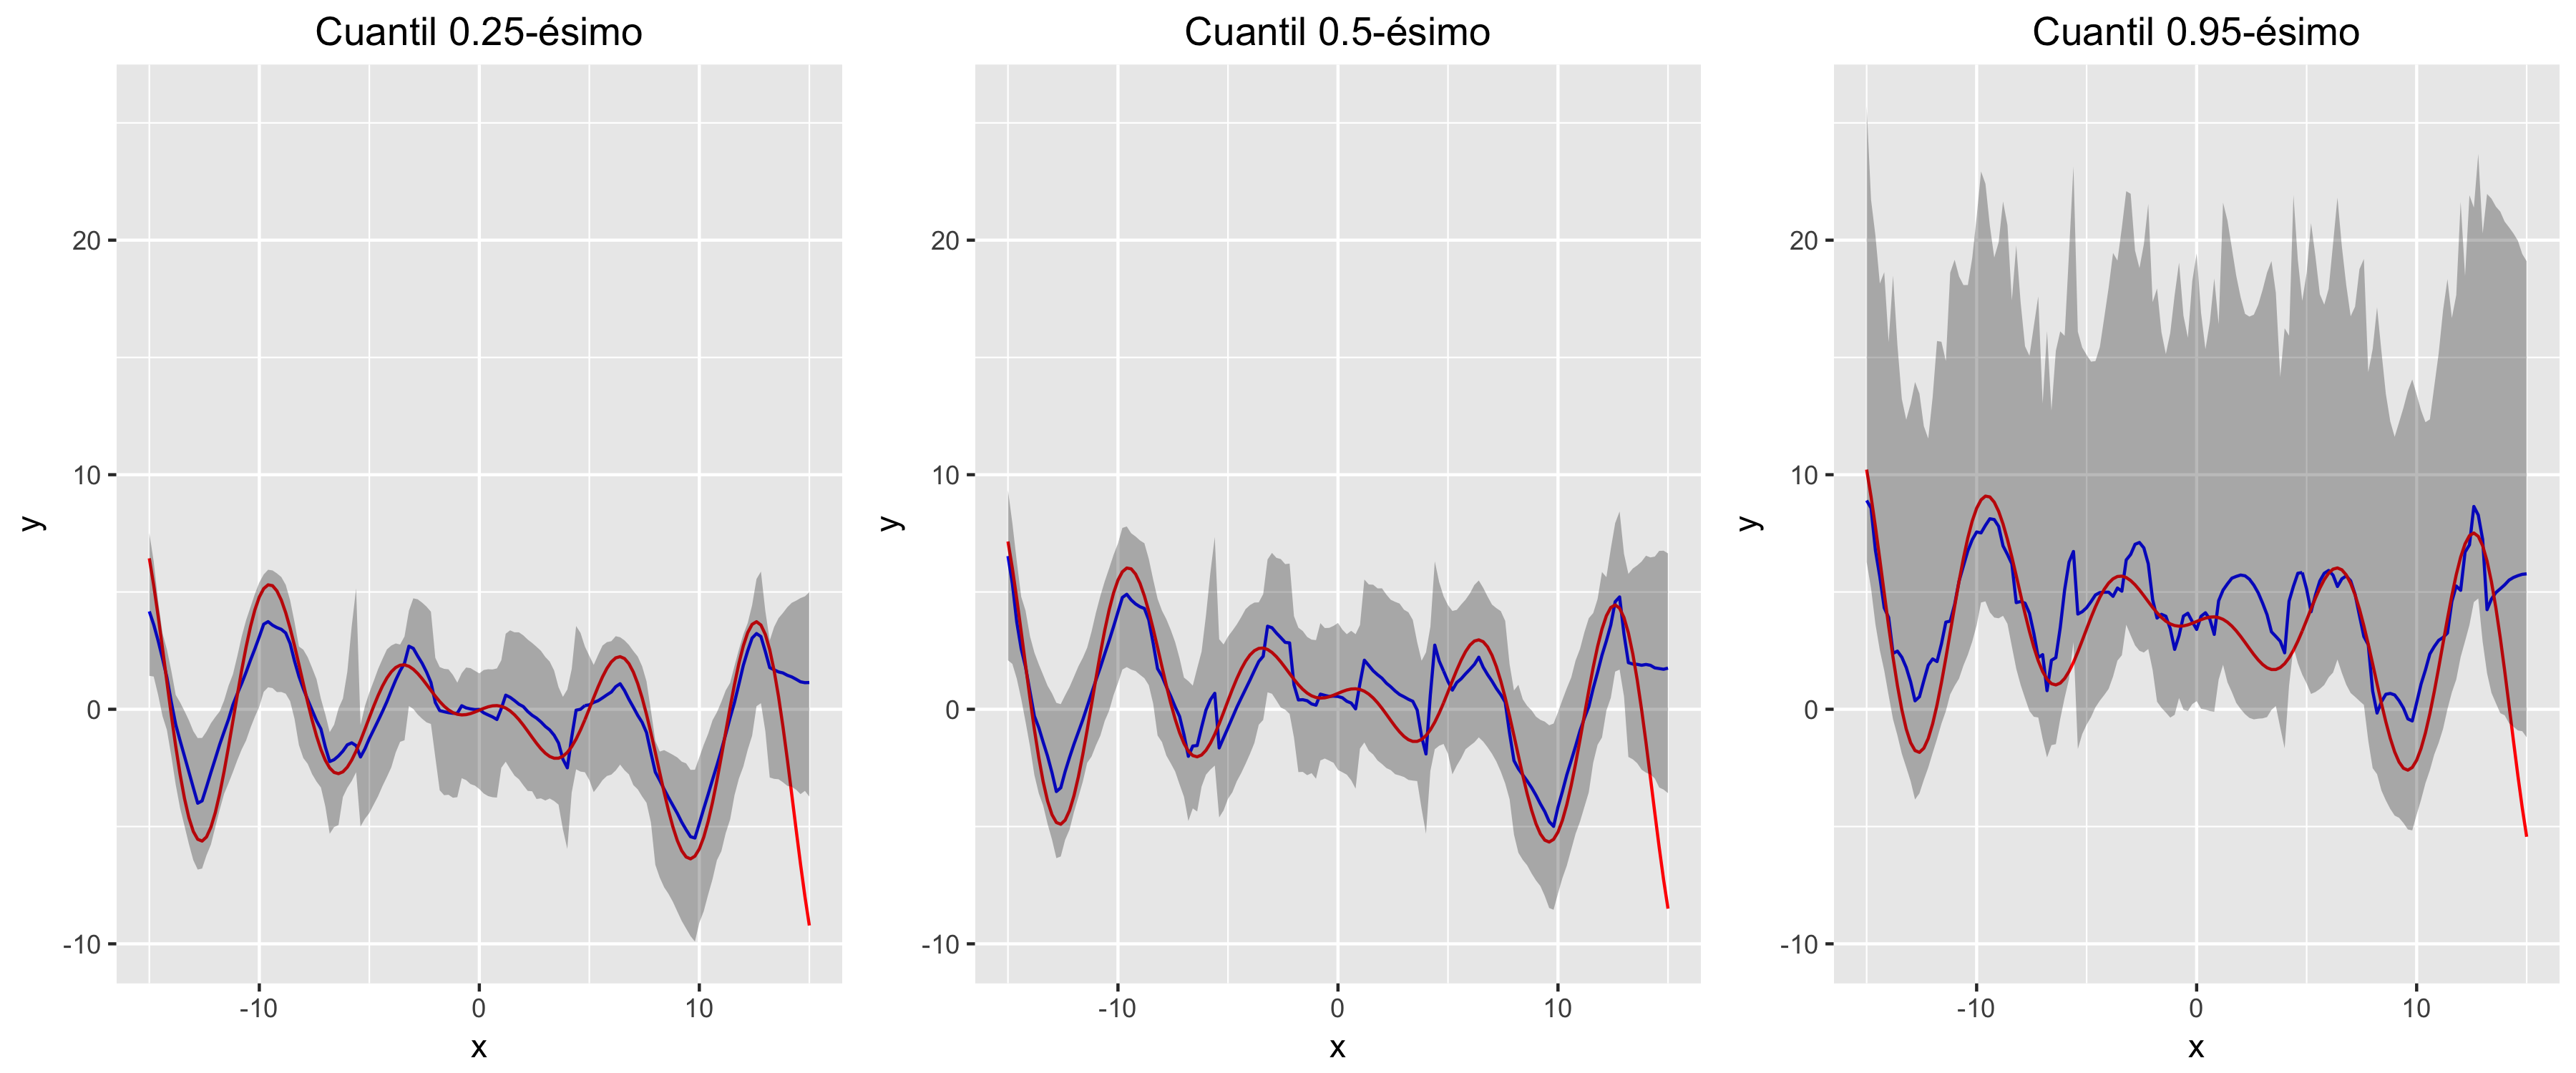
\includegraphics[width=\textwidth]{Figures/Simulation/complex_g_complex_error/fitted_models.png}
	\captionsetup{singlelinecheck=off,font=footnotesize}
    \caption*{Nota: La l\'inea roja representa el valor real de cada cuantil, la l\'inea azul representa la mediana de la distribuci\'on posterior predictiva y el \'area gris su intervalo de probabilidad al 90\%.}
	\label{fitted_cgce}
\end{figure}

Una vez corroborado que el modelo funciona bien con datos simulados, a continuaci\'on se presentan los resultados de su aplicaci\'on a un problema real, dentro de las tareas laborales del autor.

\section{Investigaci\'on de mercados}

\subsection{Conceptos iniciales}

En el contexto de la investigaci\'on de mercados una de las m\'etricas que se consideran m\'as importantes es la del \textit{conocimiento de marca}, misma que se define como el porcentaje de una cierta poblaci\'on que declara conocer el nombre de la marca en cuesti\'on.

Dentro de dicho ambiente, la teor\'ia dice que esa m\'etrica normalmente depende de la publicidad pautada semana a semana. Cuando una marca \'unicamente se publicita en televisi\'on, el valor com\'unmente usado para medir esa inversi\'on se denomina \textit{adstocked GRP}s, y, en esencia, se compone de cu\'antas veces se transmiti\'o el comercial y cu\'anta gente estaba viendo la televisi\'on cuando se transmiti\'o,  ponderado por qu\'e tan lejana en el tiempo sucedi\'o dicha transmisi\'on, respecto al d\'ia de hoy. Asimismo, tambi\'en se suelen usar las inversiones de los competidores para explicar el \textit{conocimiento de marca}, debido a que es com\'un que las personas se confundan y asocien a la marca un comercial del competidor.

En el pasado, inversiones iguales han representado resultados ligeramente distintos en los niveles de \textit{conocimiento de marca}, volatilidad que normalmente es asociada a la calidad de los comerciales, tanto los propios, como los del competidor. En otras palabras, comerciales m\'as memorables han generado un mayor \textit{conocimiento de marca} a la que los pauta, y una aportaci\'on muy pequeña al competidor, cuando se han transmitido en aproximadamente la misma cantidad ocasiones y a una similar audiencia.

Adem\'as, tambi\'en es importante revisar el concepto de \textit{marca madre} y \textit{subvariantes}, para nuestra siguiente aplicaci\'on del modelo GPDP. Una \textit{marca madre} es aquella que tiene fama por su propio nombre, pero que se ofrece al consumidor mediante productos (tambi\'en llamados \textit{subvariantes}) que son publicitados por s\'i solos. Por ejemplo, se puede pensar en la empresa de tecnolog\'ia \textit{Pera} que tiene comerciales que posicionan su nombre, pero tiene tambi\'en comerciales donde promociona \'unicamente el celular que producen, y en otros, \'unicamente la tableta.

Dicho esto, normalmente se piensa que los comerciales de la \textit{marca madre} contribuyen m\'as al \textit{conocimiento de marca} que aquellos de las \textit{subvariantes}, que tienen como prop\'osito vender los productos espec\'ificos, m\'as que posicionar la marca.

\subsection{Caso real}

Cierta \textit{marca madre} es cliente de la empresa de investigaci\'on de mercados en la que sol\'ia trabajar. Dicha marca registr\'o semana a semana los valores de inversi\'on en los comerciales que buscaban posicionar su nombre, los realizados para los de sus \textit{subvariantes}, los de su competencia y el \textit{conocimiento de marca} reportado durante 2014 y 2015. Estos sirvieron para entrenar un modelo GPDP, bajo el supuesto que las mediciones semanales fueron independientes condicionalmente a la inversi\'on. Los valores predichos por el GPDP comparados contra los que en efecto se observaron se presentan a continuaci\'on.

\begin{figure}[H]
	\centering
	\caption{Modelo de \textit{conocimiento de marca} para datos de entrenamiento (2014-2015).}
	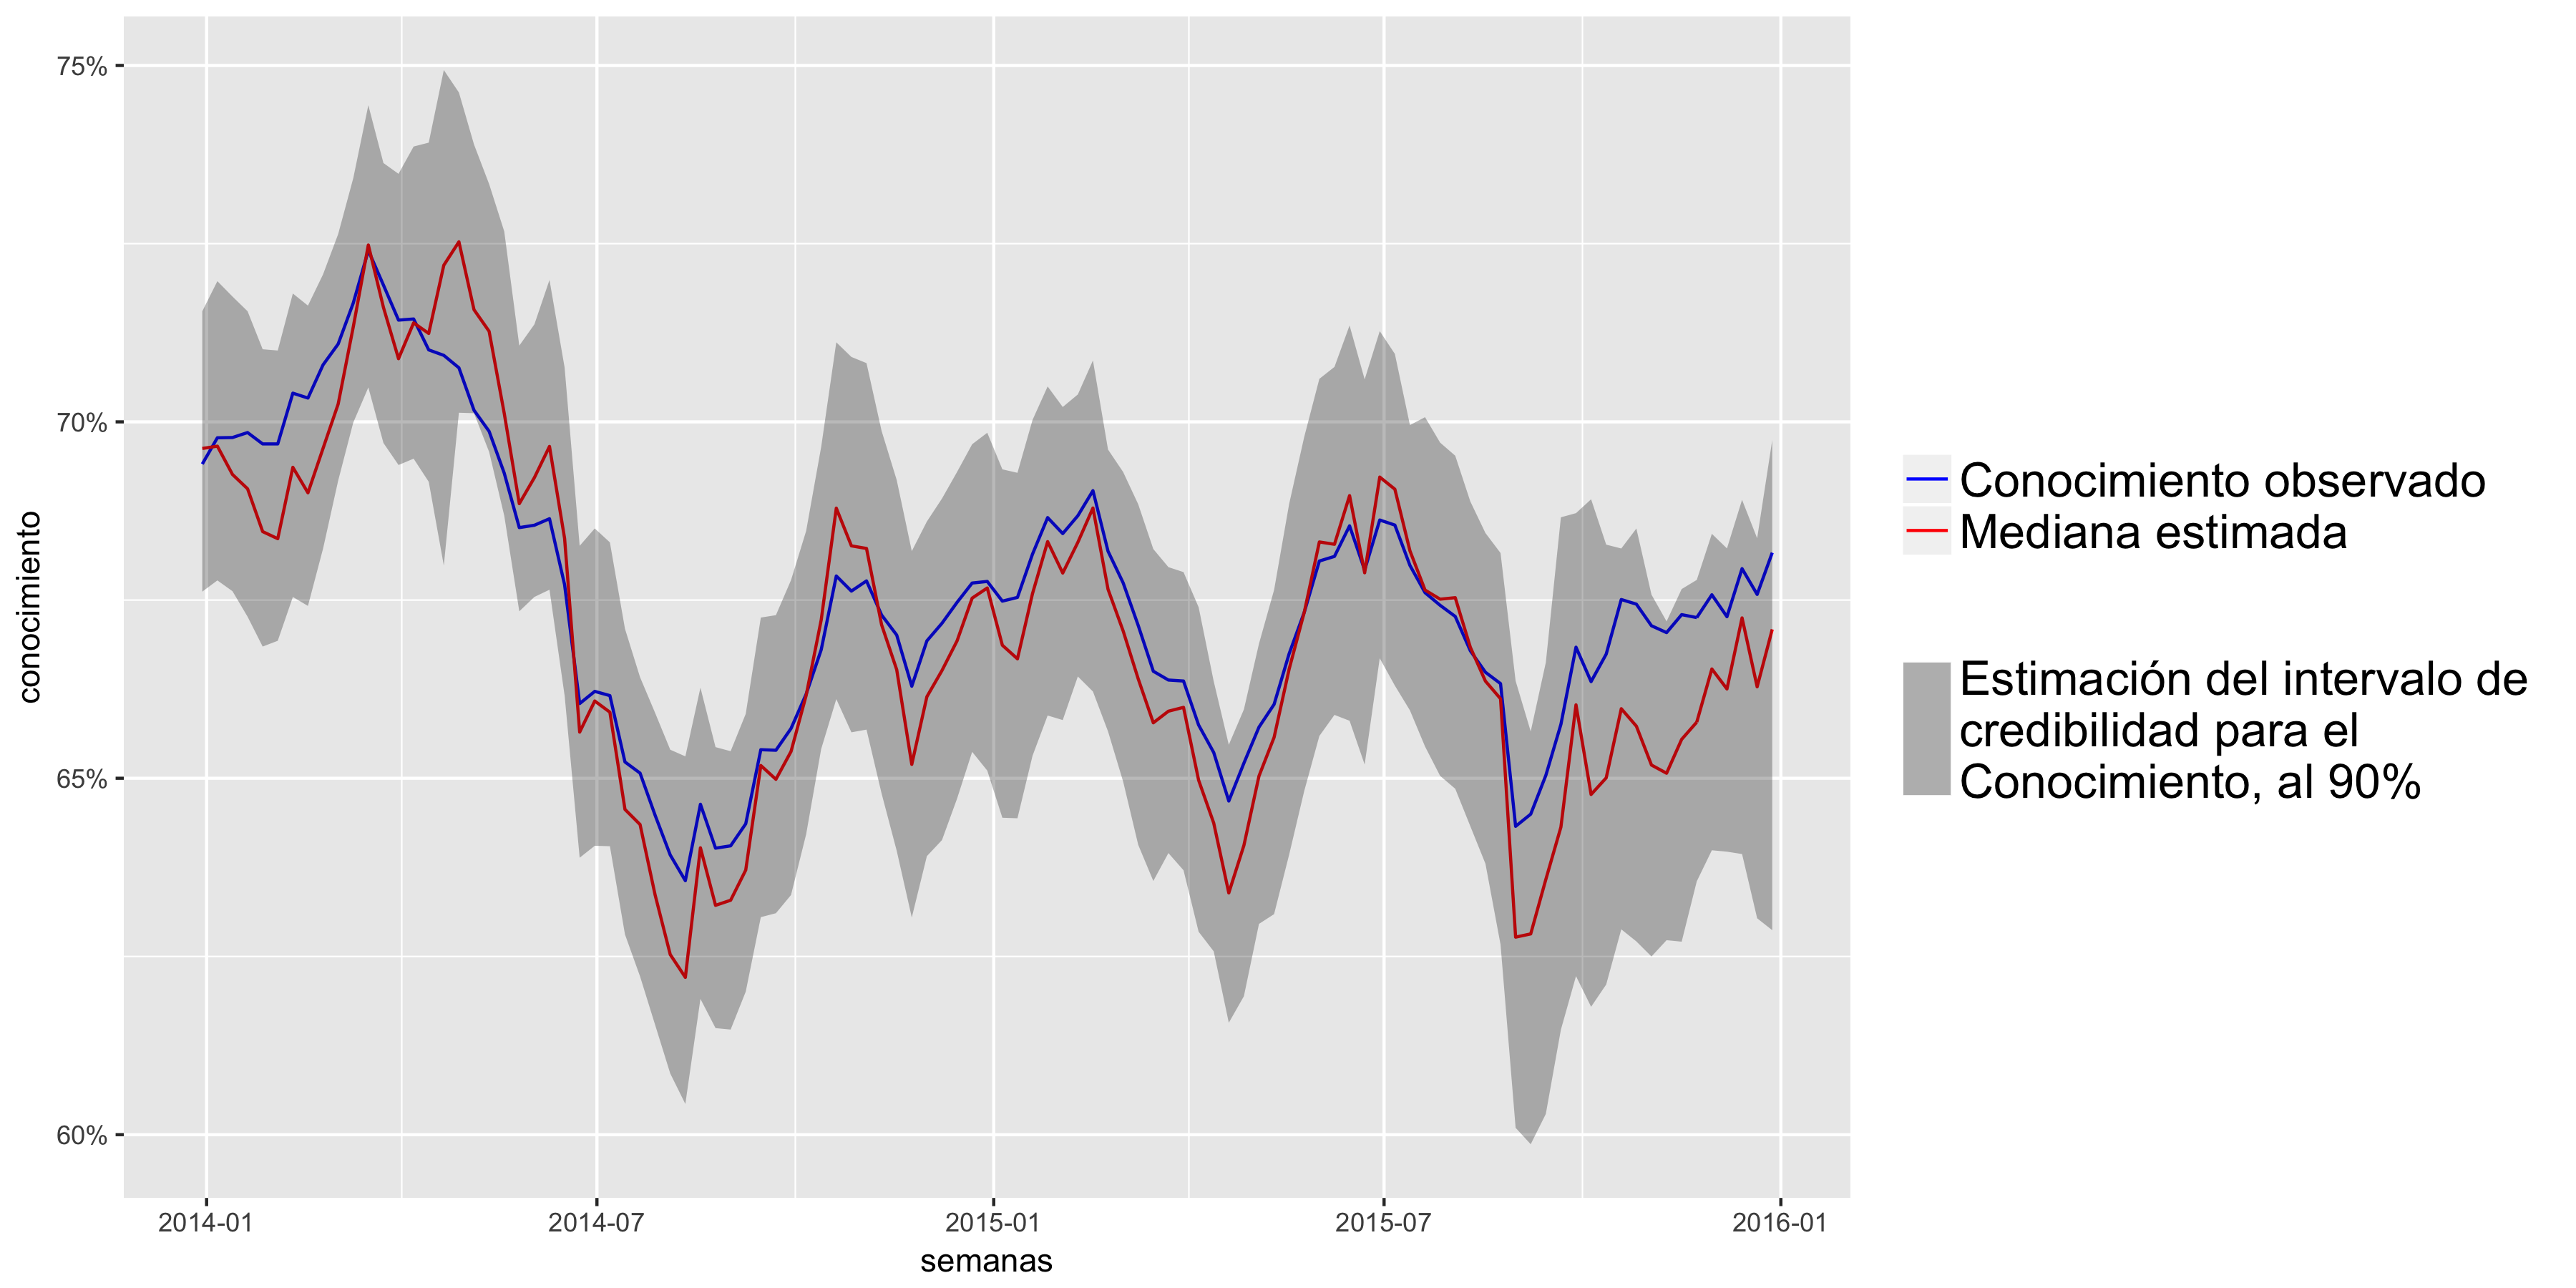
\includegraphics[width=1\textwidth]{Figures/MarketResearch/fit_review.png}
	\captionsetup{singlelinecheck=off,font=footnotesize}
	\caption*{Nota: El intervalo de credibilidad se construy\'o usando las estimaciones de la mediana de los cuantiles $0.05$-\'esimo y $0.95$-\'esimo.}
	\label{awareness_fit}
\end{figure}

Es verificable que el \textit{conocimiento de marca} sigue un movimiento muy similar a la mediana que predijo el modelo durante el primer año y medio, y, de hecho, en los \'ultimos se ha despegado positivamente.

Todo lo anterior se hizo ignorando el hecho de que tambi\'en se ten\'ian los datos de 2016, con la intenci\'on de ver c\'omo funcionar\'ia el modelo. Al cliente particularmente le interesaba ver esto porque la m\'etrica tuvo una estrepitosa ca\'ida durante el 2016 y ten\'ia la duda si era por una estrategia desafortunada de su inversi\'on o por el hecho de que su competidor hab\'ia cambiado completamente el concepto de sus comerciales, situaci\'on que podr\'ia estar provocando que la gente ya no se confundiera y los relacionara err\'oneamente a los de la marca de nuestro cliente.

Traslado al lenguaje del modelo, se deseaba ver si el valor realmente observado pudo haber sido predicho por el modelo o si lo consideraba poco probable, situaci\'on en la que efectivamente se podr\'ia hablar de un cambio estructural ocurrido dentro de este contexto. Los resultados obtenidos fueron los siguientes.

\begin{figure}[H]
	\centering
	\caption{\textit{Conocimiento de marca} en 2016, comparado con el modelo GPDP.}
	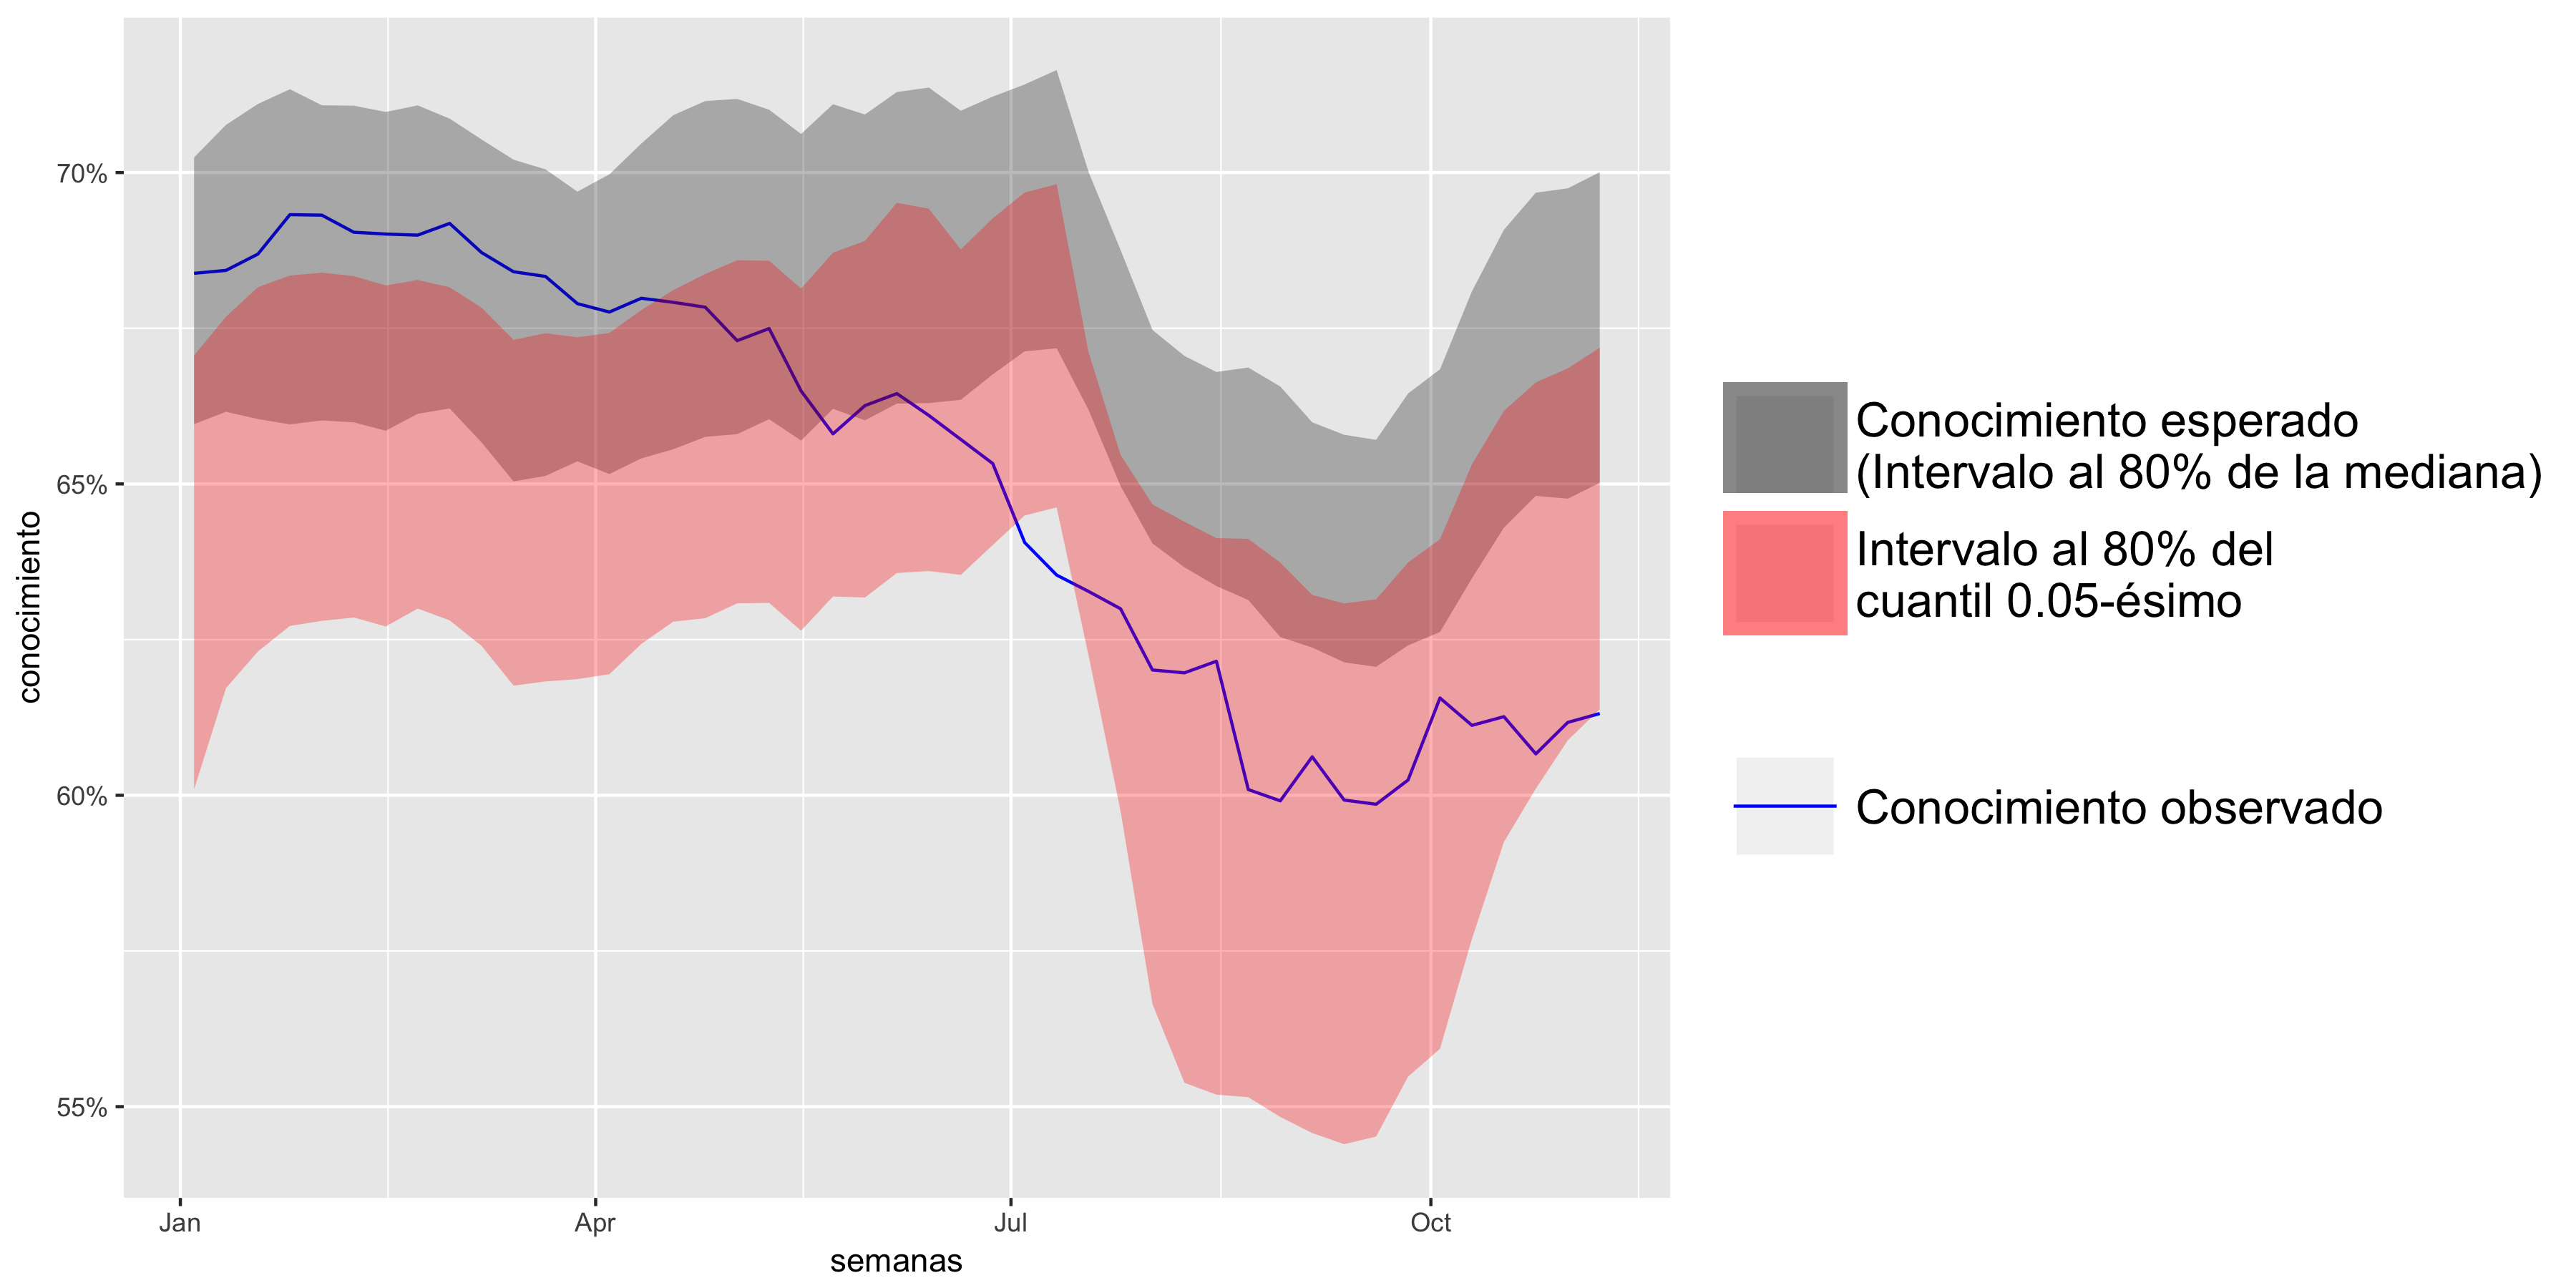
\includegraphics[width=1\textwidth]{Figures/MarketResearch/goals_2016.png}
	\captionsetup{singlelinecheck=off,font=footnotesize}
	\label{awareness_fit}
\end{figure}

Como se puede observar, hasta el mes de abril el \textit{conocimiento de marca} se comport\'o de acuerdo a lo esperado, pero despu\'es tuvo una ca\'ida estrepitosa que, si bien el modelo hab\'ia anticipado para despu\'es de julio, coincidi\'o en mayor medida con lo que se hubiera esperado para el cuantil $0.05$-\'esimo. Es decir, suponiendo que no hubiera cambio estructural, se habr\'ia presenciado el peor de cada 20 casos.

En otras palabras, confiando en la construcci\'on del modelo, el supuesto de independencia entre las observaciones y un error modesto en la medici\'on del \textit{conocimiento de marca}, hay informaci\'on suficiente para pensar que, en efecto, el cambio de concepto en los comerciales del competidor impact\'o la m\'etrica del cliente.


\newpage